\documentclass[preprint2]{aastex}
\usepackage[colorlinks]{hyperref}
\usepackage{amsmath, bm}
\usepackage{fancyhdr}
\usepackage{floatrow}
\usepackage[inner=2cm,outer=2cm,bottom=1cm,top=1.5cm]{geometry}
\usepackage{mathtools}
\usepackage{multicol}
\usepackage{verbatim}
\usepackage{graphicx,float,wrapfig, subcaption}
\usepackage{indentfirst}
\usepackage{soul}

\newcommand{\Ibar}{\mbox{\st{$I$}}}

\newcommand{\deri}[2]{\frac{\mathrm{d} #1}{\mathrm{d} #2}}
\newcommand{\inte}[4]{\int_{#1}^{#2} \! #3 \, \mathrm{d} #4}

\fancyhf{} % clear all header and footers
\renewcommand{\headrulewidth}{0pt} % remove the header rule
\rhead{\thepage}

%
%lfoot{\thepage} % puts it on the left side instead
%
% or if your document is 2 sided, and you want even and odd placement of the number
%facncyfoot[LE,RO]{\thepage} % Left side on Even pages; Right side on Odd pages
%
\pagestyle{fancy}

\begin{document}

\title{Newtonian Binary Coalescence}

\author{\vspace{-0.5cm}{\sc John Pharo}\email{jpharo@caltech.edu}\vspace{0.2cm}{\sc Cutter Coryell}\email{ccoryell@caltech.edu}
\vspace{0.2cm}\affil{California Institute of Technology} \vspace{1cm}}



\section{Introduction}

In the paper \textit{Gravitational Radiation and the Motion of Two Point Masses} (Peters 1964), the equations of general relativity are used to obtain equations of conservation of energy, momentum, and angular momentum. From this, Peters determines the energy loss and angular momentum loss of a binary system of compact objects due to radiating gravitational waves. This yields the equations
\[ \frac{dE}{dt} = \frac{G}{5c^5} \left( \frac{\partial^3 \Ibar_{ij}}{\partial t^3} \right)^2 \hspace*{0.5cm} \frac{dL_z}{dt} = \frac{2G}{5c^5} \epsilon_{zjk} \left( \frac{\partial^2 \Ibar_{ij}}{\partial t^2} \frac{\partial^3 \Ibar_{km}}{\partial t^3} \right) \]
where \(\Ibar\) is the reduced quadrupole tensor (with separation vector \(\vec{x} (t)\) and reduced mass $\mu$):

\begin{equation} \label{quad}
\Ibar_{ij}  =\mu (x_i x_j - \frac{1}{3} \delta_{ij} x_k x_k)
\end{equation}

The purpose of this project is to simulate the orbit and gravitational wave production of such a binary system. This can be done through numerical evaluation of the eccentricity and semi-major axis of the system. Derived in Peters Equations 5.6 and 5.7 for binaries with object masses \(m_1\) and \(m_2\) and total mass~\(M\):

\begin{equation} \label{axis}
\left< \frac{da}{dt} \right> = - \frac{64}{5} \cdot \frac{G^3 m_1 m_2 M}{c^5 a^3 (1 - e^2)^{7/2}} \left( 1 + \frac{73}{24} e^2 + \frac{37}{96} e^4 \right)
\end{equation}

\begin{equation} \label{ecc}
\left< \frac{de}{dt} \right> = - \frac{304}{15} \cdot e \cdot \frac{G^3 m_1 m_2 M}{c^5 a^4 (1 - e^2)^{5/2}} \left( 1 + \frac{121}{304}e^2 \right)
\end{equation}

Furthermore, we may write the evolution of the true anomaly \(\phi\) in terms of \(a\), \(e\), and \(r\):

\[
 \frac{d \phi}{dt} = \frac{L}{r^2}
\]
\[
a(1 - e^2) = \frac{L^2}{GM}
\]
\begin{equation} \label{phi}
\implies \frac{d \phi}{dt} = \frac{\sqrt{GMa(1 - e^2)}}{r^2}
\end{equation}

Through the use of Runge-Kutta integration, we may numerically evaluate \eqref{axis}, \eqref{ecc}, and \eqref{phi} in order to track the orbit of the system over time. From the values of \(a\) and \(e\), the angular momentum \(L\) and the energy \(E\) can be calculated:

\begin{equation} \label{momentum}
a(1 - e^2) = \frac{L^2}{GM} \implies L = \sqrt{GMa(1 - e^2)}
\end{equation}
\begin{equation} \label{energy}
e = \sqrt{1 + \frac{2EL^2}{(GM)^2}} \implies E = \frac{1}{2} \left( \frac{G M}{L} \right)^2 (e^2 - 1)
\end{equation}

Furthermore, by computing the separation vector via the value of \(\phi\) and
\begin{equation} \label{r}
r(\phi) = \frac{a(1-e^2)}{1 + e \cos(\phi)}
\end{equation}
one can track the change in the reduced quadrupole over time via \eqref{quad}, which can be used to find the plus-polarized and cross-polarized gravitational wave strains via

\begin{equation} \label{hplus}
h_+ = \frac{G}{c^4} \left( \frac{\ddot{\Ibar}_{xx} - \ddot{\Ibar}_{yy}}{r} \right)
\end{equation}
\begin{equation} \label{hcross}
 h_{\times} = \frac{2G}{c^4} \frac{\ddot{\Ibar}_{xy}}{r}
\end{equation}

\section{The Code}

This project uses two main sections of code, one for the actual simulation of the binary system and one for analysis and production of plots of the data.

\subsection{Simulation}

The simulation code \texttt{simulate.py} is responsible for numerically evolving the binary system's orbital parameters and generating the simulated orbits and gravitational wave strains over a given time scale.

The first section of the code sets various constants and parameters for the system. This includes the initial data settings for simulating the current Hulse-Taylor binary and several important parameters for running the simulation. Of particular importance here are the names of the output and input directories (the latter is used if the simulation is being continued from a previous run), the duration of the simulation in simulated time, and the number of time steps used in the simulation (these last two determined the fixed time-step size).

The next two sections are a series of helper functions and the main code body itself. The main code begins by either opening a previous simulation to continue where it left off, or by establishing a new set of initial conditions for a new simulation. This done, the code enters the main loop of the program, which will terminate upon reaching the end of the  number of time steps.

First, the loop calls a helper function to perform RK4 integration of \eqref{axis}, \eqref{ecc}, and \eqref{phi}. The RK4 integrator itself uses several helper functions, each representing the right-hand side of the equations presented in the Introduction. Having calculated the values of $a$, $e$, and $\phi$ at the current time, the code then calls helper functions to calculate the new separation vector via~\eqref{r} and reduced quadrupole tensor via~\eqref{quad}, and from these it calculates the wave strains via \eqref{hplus}~and~\eqref{hcross}.

The code can be set to produce a 3-D movie of the orbit as it is computed; if so, it is at this point in the code that the movie updates. However, it should be noted that running the display slows the simulation down significantly. After this, the loop pickles the current state of the simulation and outputs it to the specified output directory. Every time a specified number of iterations have passed, the loop prints an update on its progress to \texttt{stdout}. The frequencies that data is output and the movie (if shown) is updated can also be specified.

\subsection{Analysis}

The analysis code \texttt{analyze.py} is responsible for taking the output generated by the simulation and plotting it in a useful fashion. The first section sets general useful constants in CGS. The second section takes important parameters for analyzing the simulation data, especially the name of the directory containing the data to be analyzed and the number of iterations it contains.

The next two sections load the existing data into lists and then use Equations \eqref{momentum} and \eqref{energy} to calculate the angular momentum and the energy of the system, respectively.

Finally, the code generates plots of various quantities and saves them to a plot directory.

\section{Results}

\subsection{Present-Day Hulse-Taylor Binary}

Upon completing the simulation code, we first simulated the present-day PSR B1913+16 binary system, also known as the Hulse-Taylor binary, a system of two orbiting neutron stars of approximately \(1.4 M_\odot\) each. We evolved the system for \(7.2 \times 10^{4}\)~s, or 20 hours. The orbital radius and true anomaly are plotted over the course of the simulation in Figures~\ref{orbit-radius}~and~\ref{orbit-phi}, respectively. The two polarizations of the gravitational wave strain are plotted versus time in Figure~\ref{orbit-strain}. Because we evolved the simulation for such a short time, \(a\), \(e\), and consequently E and L barely change, so their plots are omitted.

\begin{figure}[H]
\vspace{-0.24cm}
\centering
\hspace*{-1cm}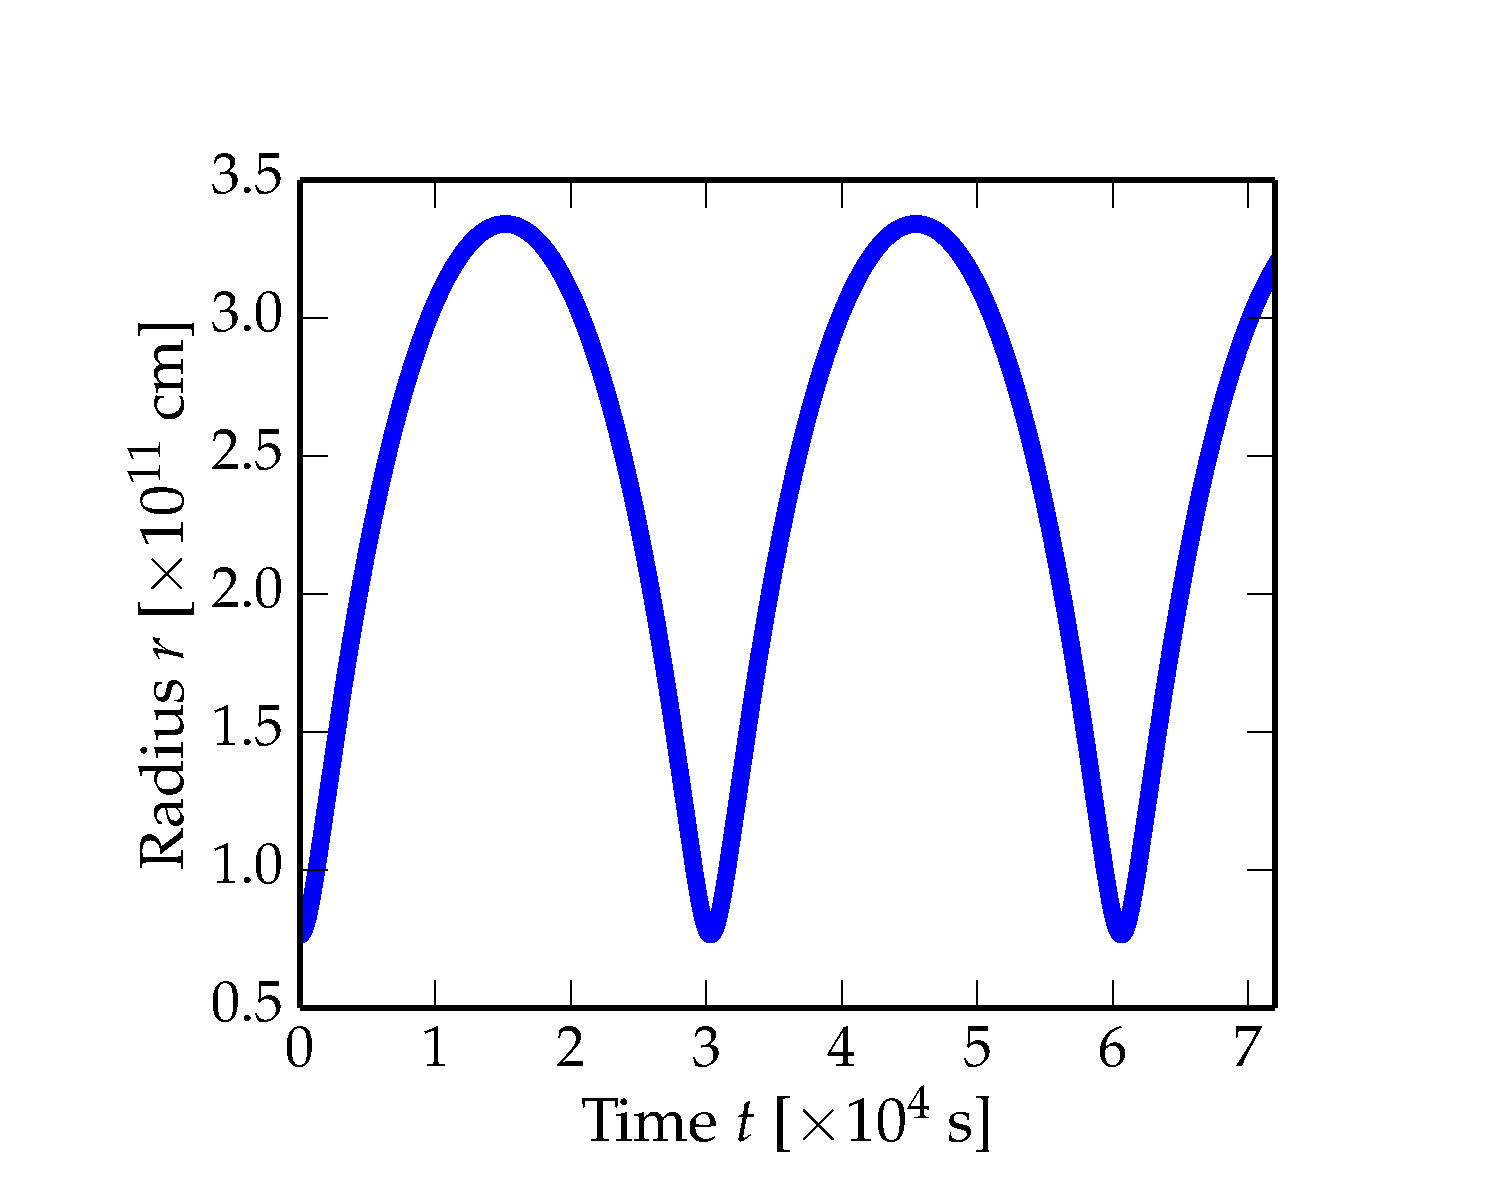
\includegraphics[width=1.2\textwidth]{orbit_figs/radius.pdf}
\caption{The radius \(r\), or orbital separation, of the Hulse-Taylor binary over a period of 20 hours. The oscillations in the separation are due to the ellipticity of the orbit.}
\label{orbit-radius}
\end{figure}
 
\begin{figure}[H]
\vspace{-0.24cm}
\centering
\hspace*{-1cm}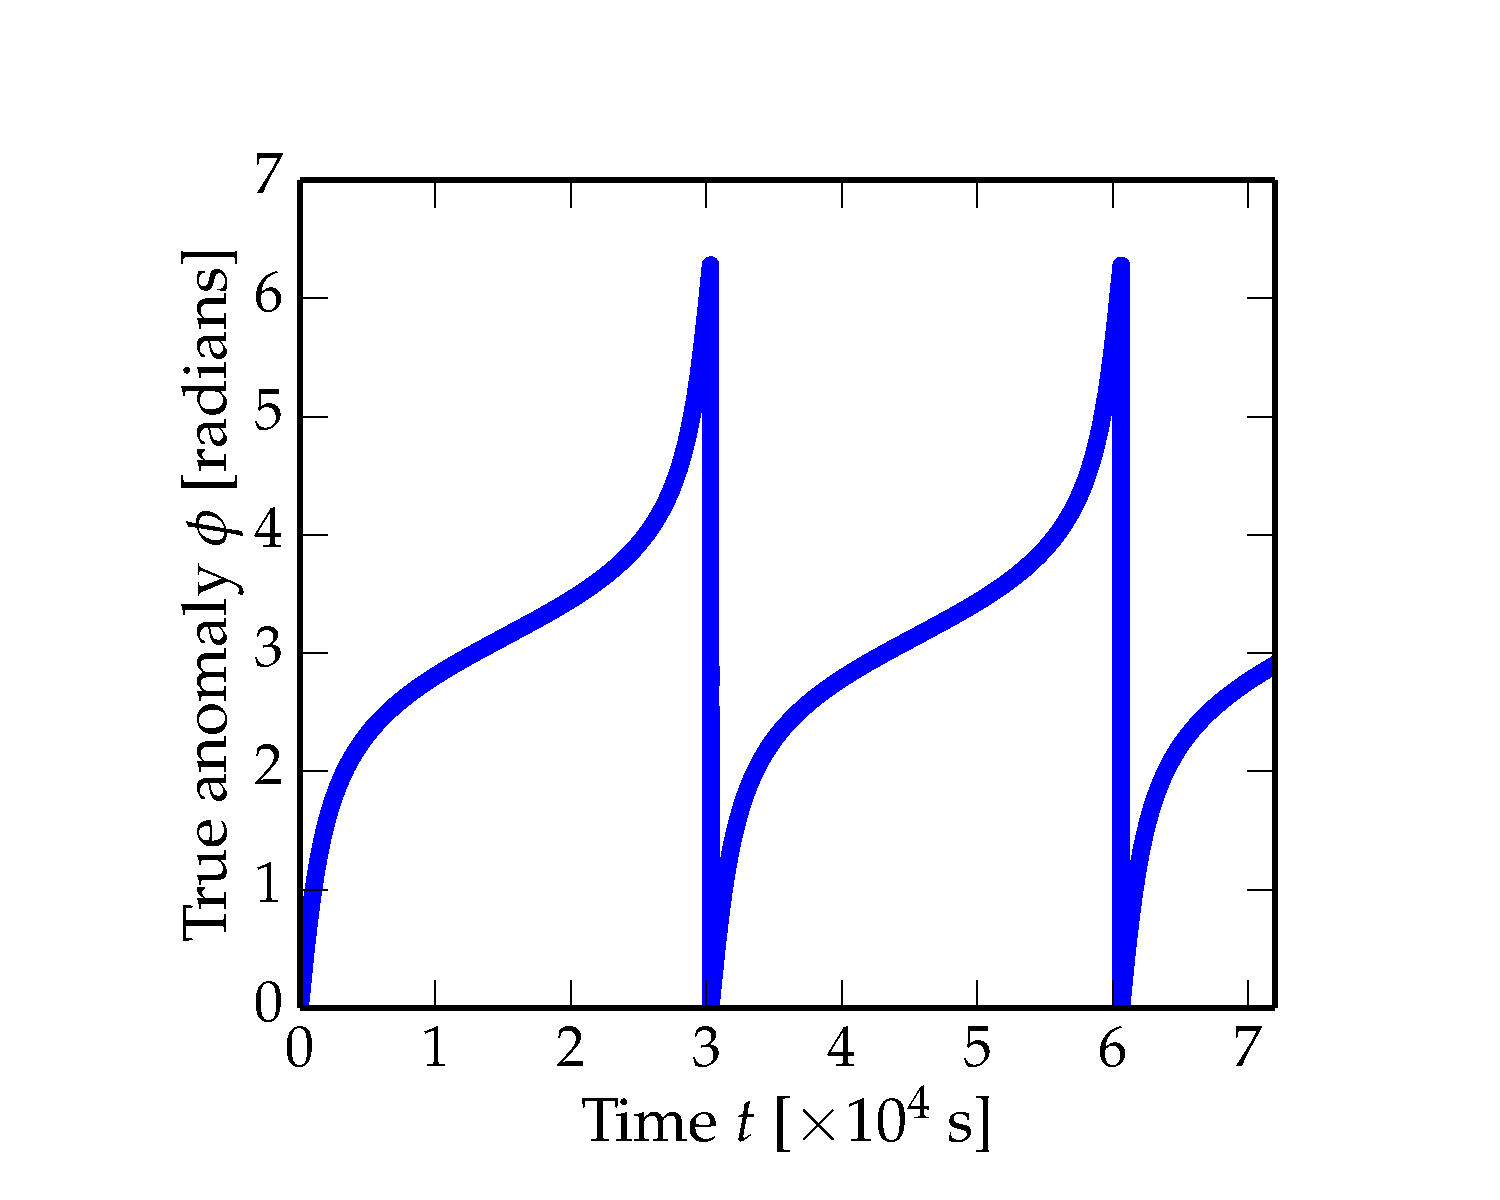
\includegraphics[width=1.2\textwidth]{orbit_figs/true-anomaly.pdf}
\caption{The true anomaly \(\phi\) of the Hulse-Taylor binary over a period of 20 hours. The true anomaly is the angle between a line connecting the center of mass of system to one of the two stars at periapsis (closest approach) and the line connecting the center of the mass to the same star at another time.}
\label{orbit-phi}
\end{figure}

\begin{figure}[t!]
\centering
\hspace*{-1cm}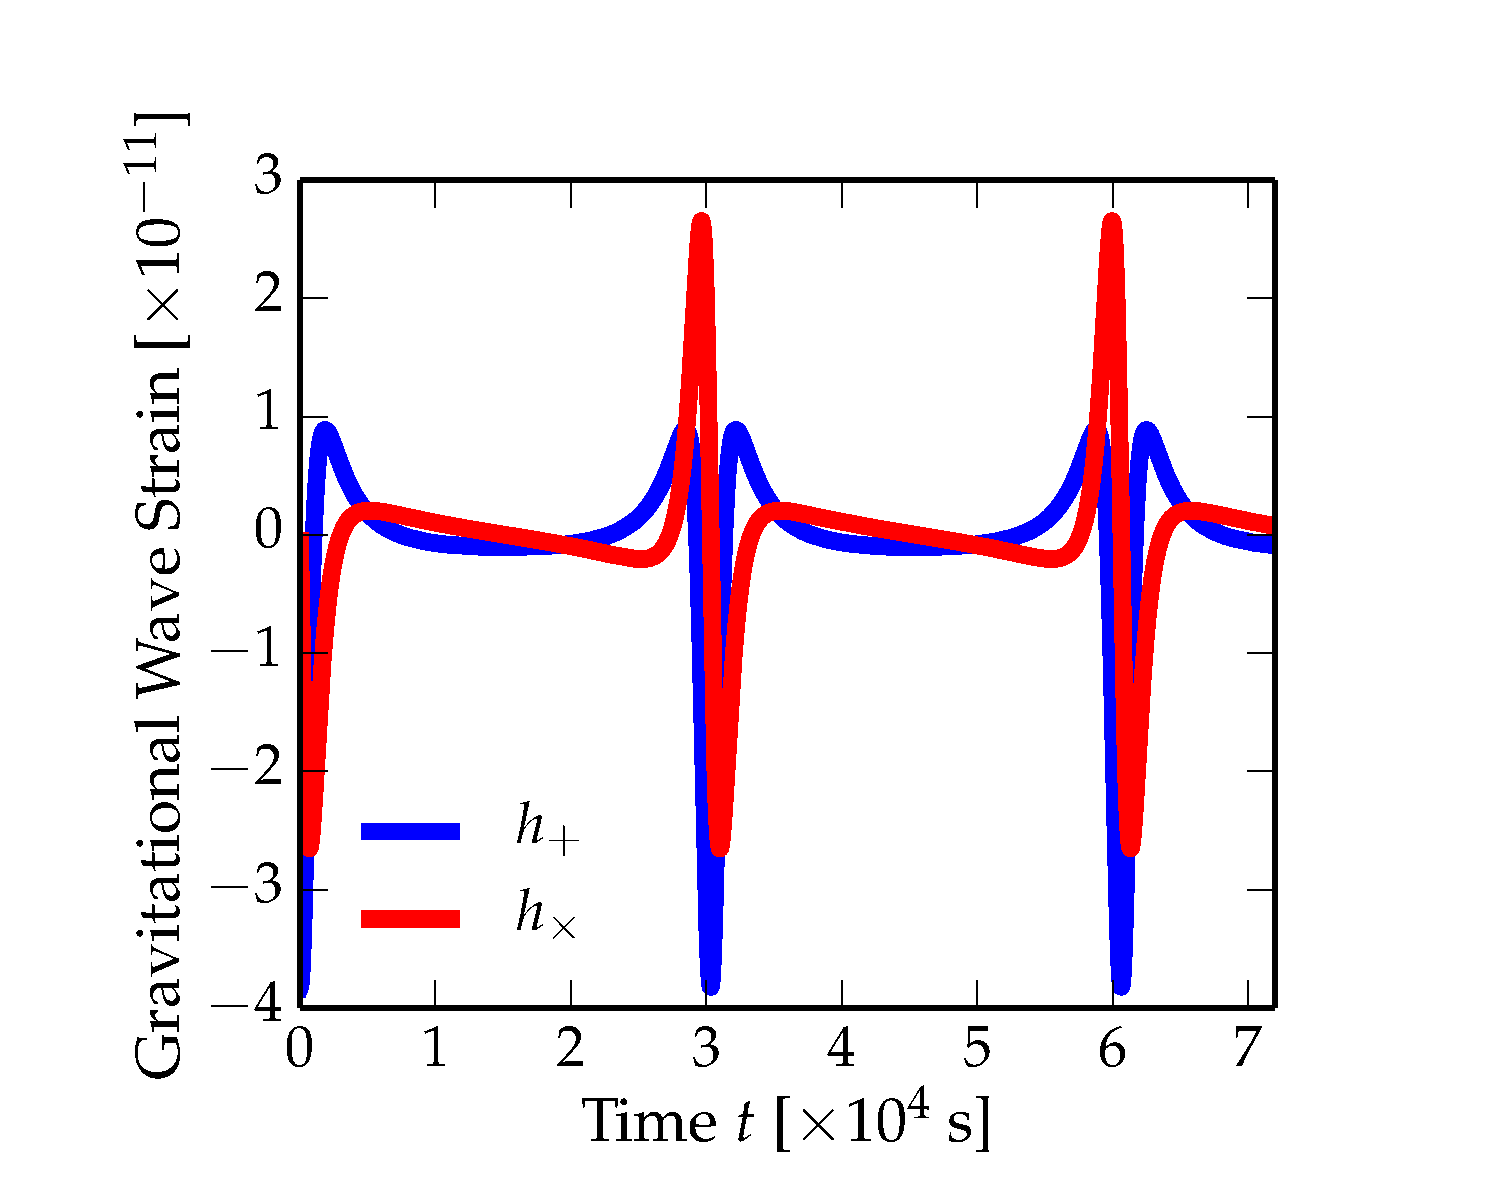
\includegraphics[width=1.2\textwidth]{orbit_figs/gw-strain.pdf}
\caption{The plus- and cross-polarized gravitational wave strain of the Hulse-Taylor binary over a period of 20 hours, or about 2.5 orbits. Comparing with Figure~\ref{orbit-radius}, we see that gravitational wave emission is most intense at the closest approach of the neutron stars.}
\label{orbit-strain}
\end{figure}

\subsection{Evolution of Hulse-Taylor Binary}

To investigate how \(a\) and \(e\) evolve in the Hulse-Taylor binary due to gravitational-wave emission, we simulated the binary one billion years into the future. Due to limitations of computing power, the time-step size was 1000 years, during which there are approximately 1 million orbits, or 1 million oscillations of \(r\) and \(\phi\). Therefore the integration of \(\phi\) will be completely wrong, but since \(a\) and \(e\) are independent of \(\phi\) and \(r\), our computation of their evolution is still valid. The results for \(a\), \(e\), and thereby \(L\) and \(E\) are plotted in Figures~\ref{billion-axis}, \ref{billion-ecc}, \ref{billion-momentum}, and \ref{billion-energy}, respectively.

\begin{figure}[t!]
\vspace{-0.24cm}
\centering
\hspace*{-1cm}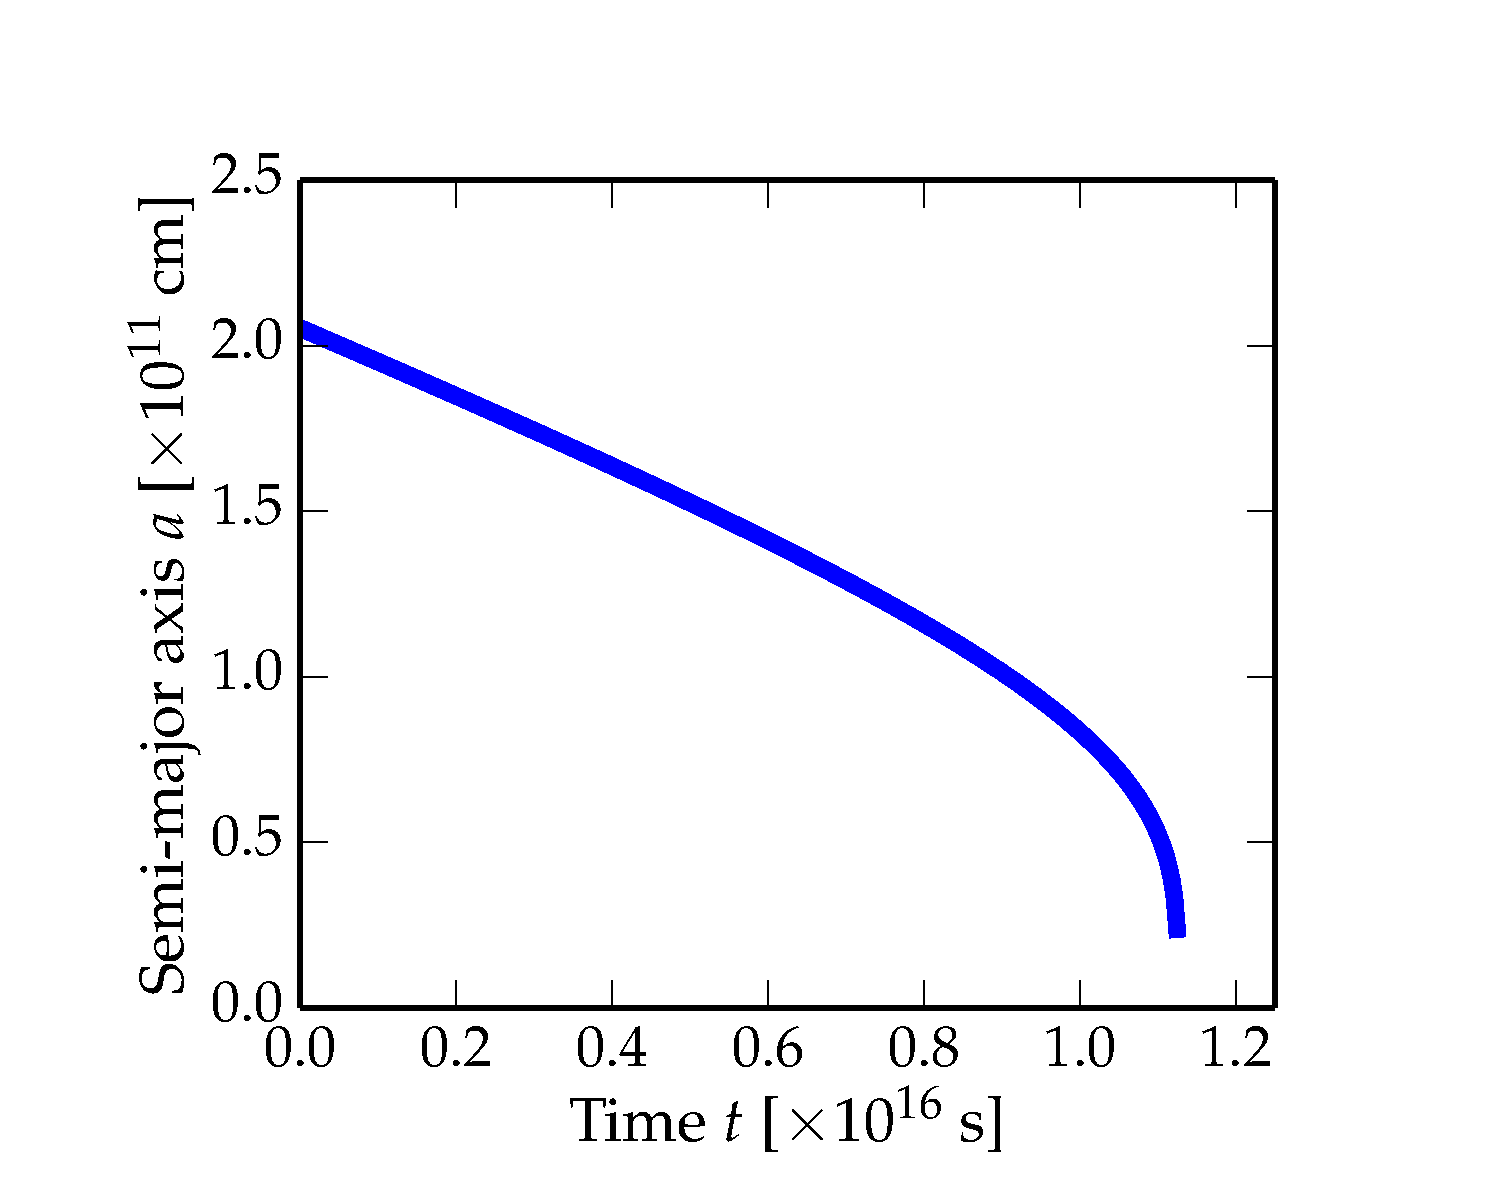
\includegraphics[width=1.2\textwidth]{billion_figs/semi-major-axis.pdf}
\caption{The semi-major axis of the Hulse-Taylor binary over the course of \(\sim\) 300 million years. The orbital separation decreases over time due to gravitational radiation. The simulation was terminated at \(1.12 \times 10^{16}\) seconds \(\sim\) 357 million years when the semi-major axis reached zero, indicating that the binary had coalesced.}
\label{billion-axis}
\end{figure}

\begin{figure}[t!]
\vspace{-0.24cm}
\centering
\hspace*{-1cm}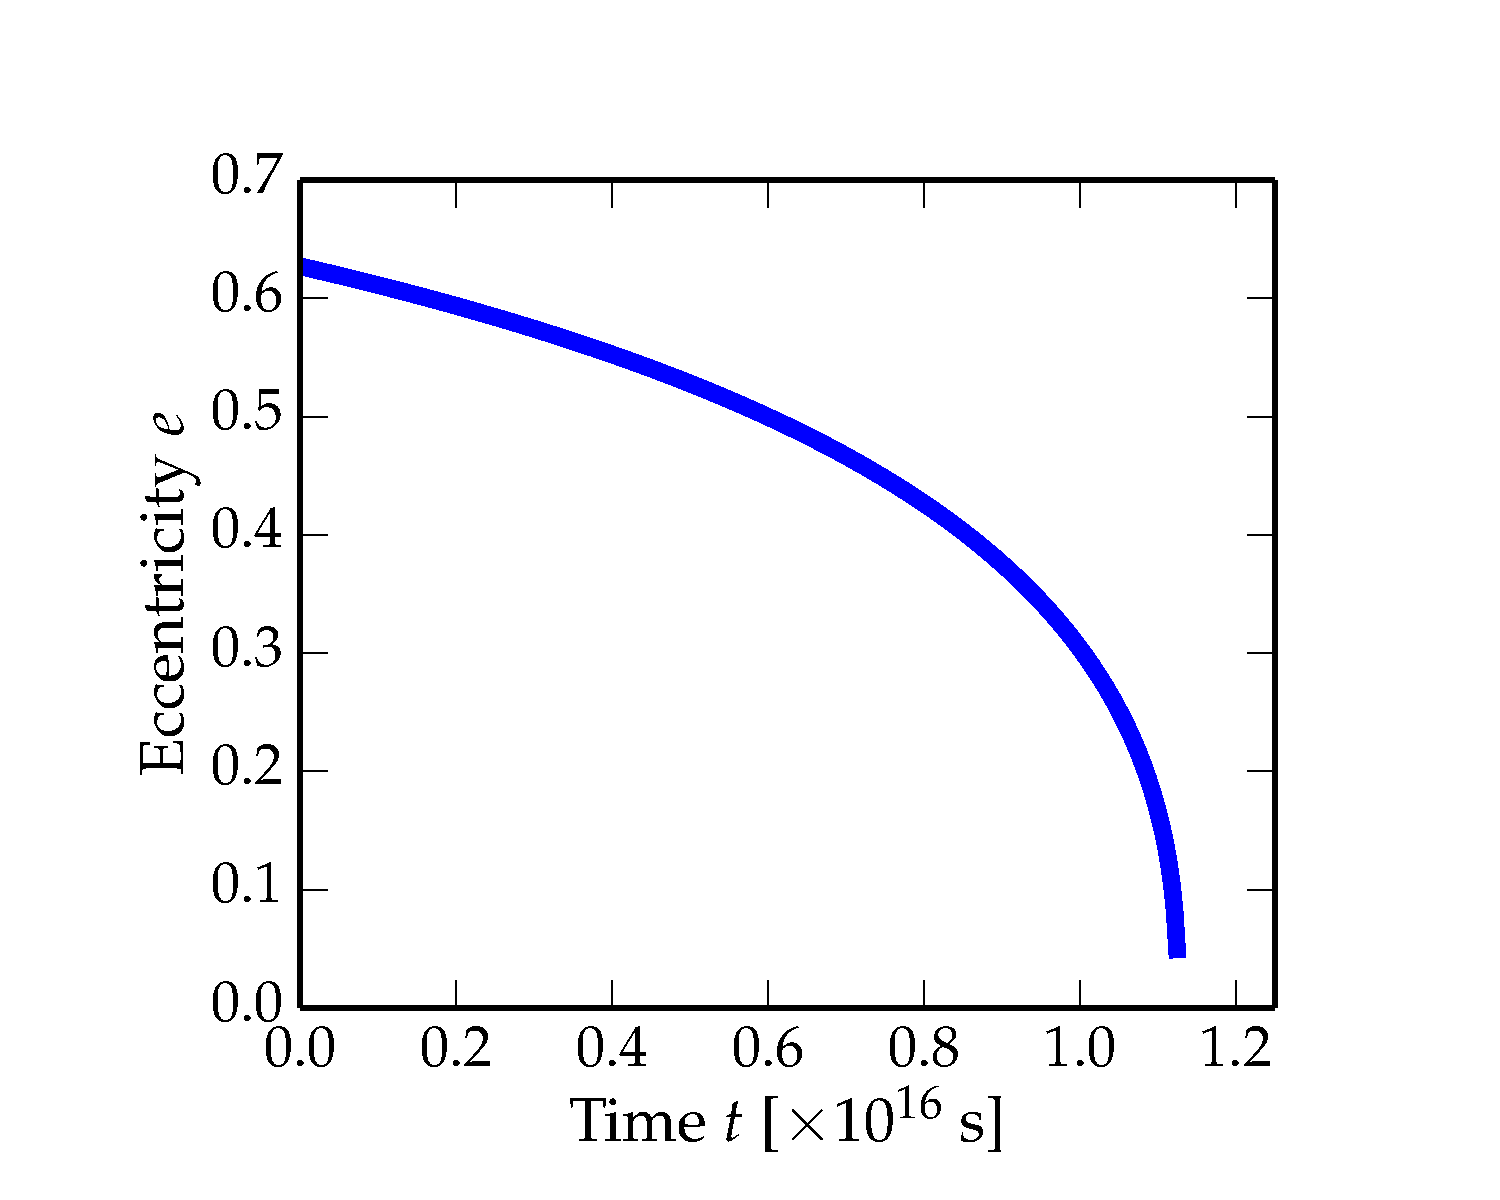
\includegraphics[width=1.2\textwidth]{billion_figs/eccentricity.pdf}
\caption{The eccentricity of the Hulse-Taylor binary over the course of \(\sim\) 300 million years. Gravitational radiation circularizes the orbits of the binary companions, more so as the binary separation decreases over time.}
\label{billion-ecc}
\end{figure}

\begin{figure}[t!]
\vspace{-0.24cm}
\centering
\hspace*{-1cm}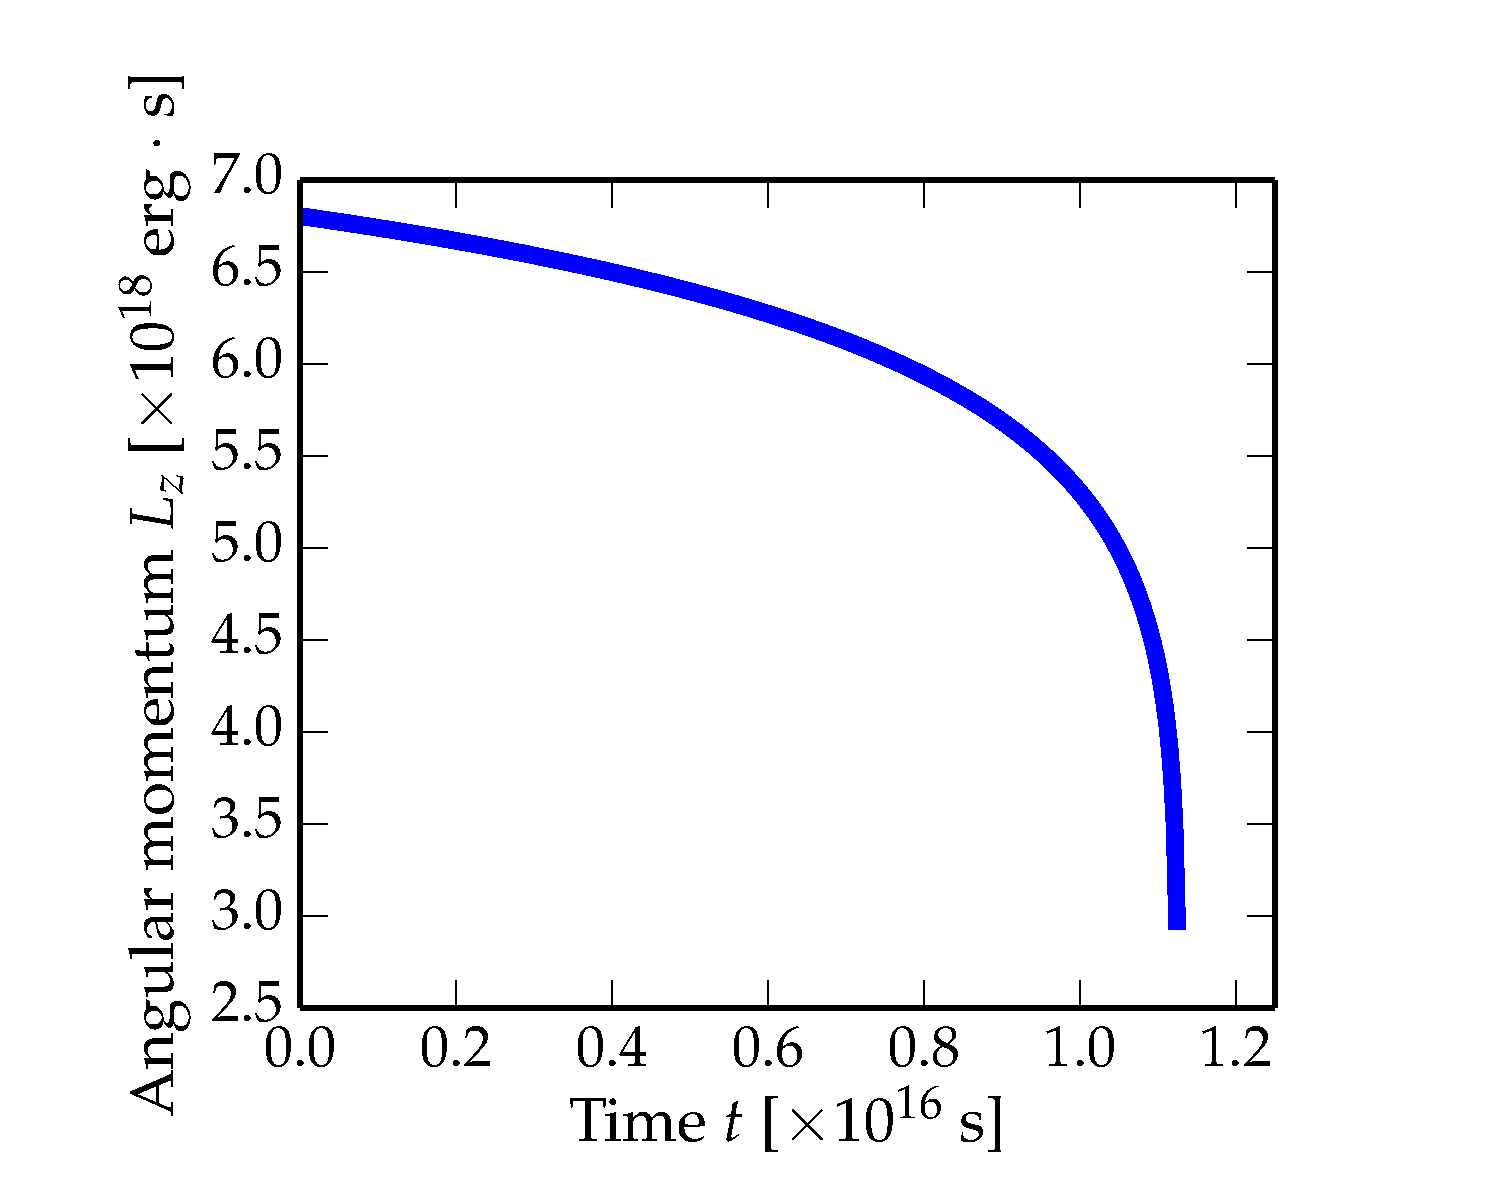
\includegraphics[width=1.2\textwidth]{billion_figs/angular_momentum.pdf}
\caption{The angular momentum of the Hulse-Taylor binary over the course of \(\sim\) 300 million years. Angular momentum is radiated away by gravitational waves at a rate that increases as the binary separation decreases over time.}
\label{billion-momentum}
\end{figure}

\begin{figure}[t!]
\vspace{-0.24cm}
\centering
\hspace*{-1cm}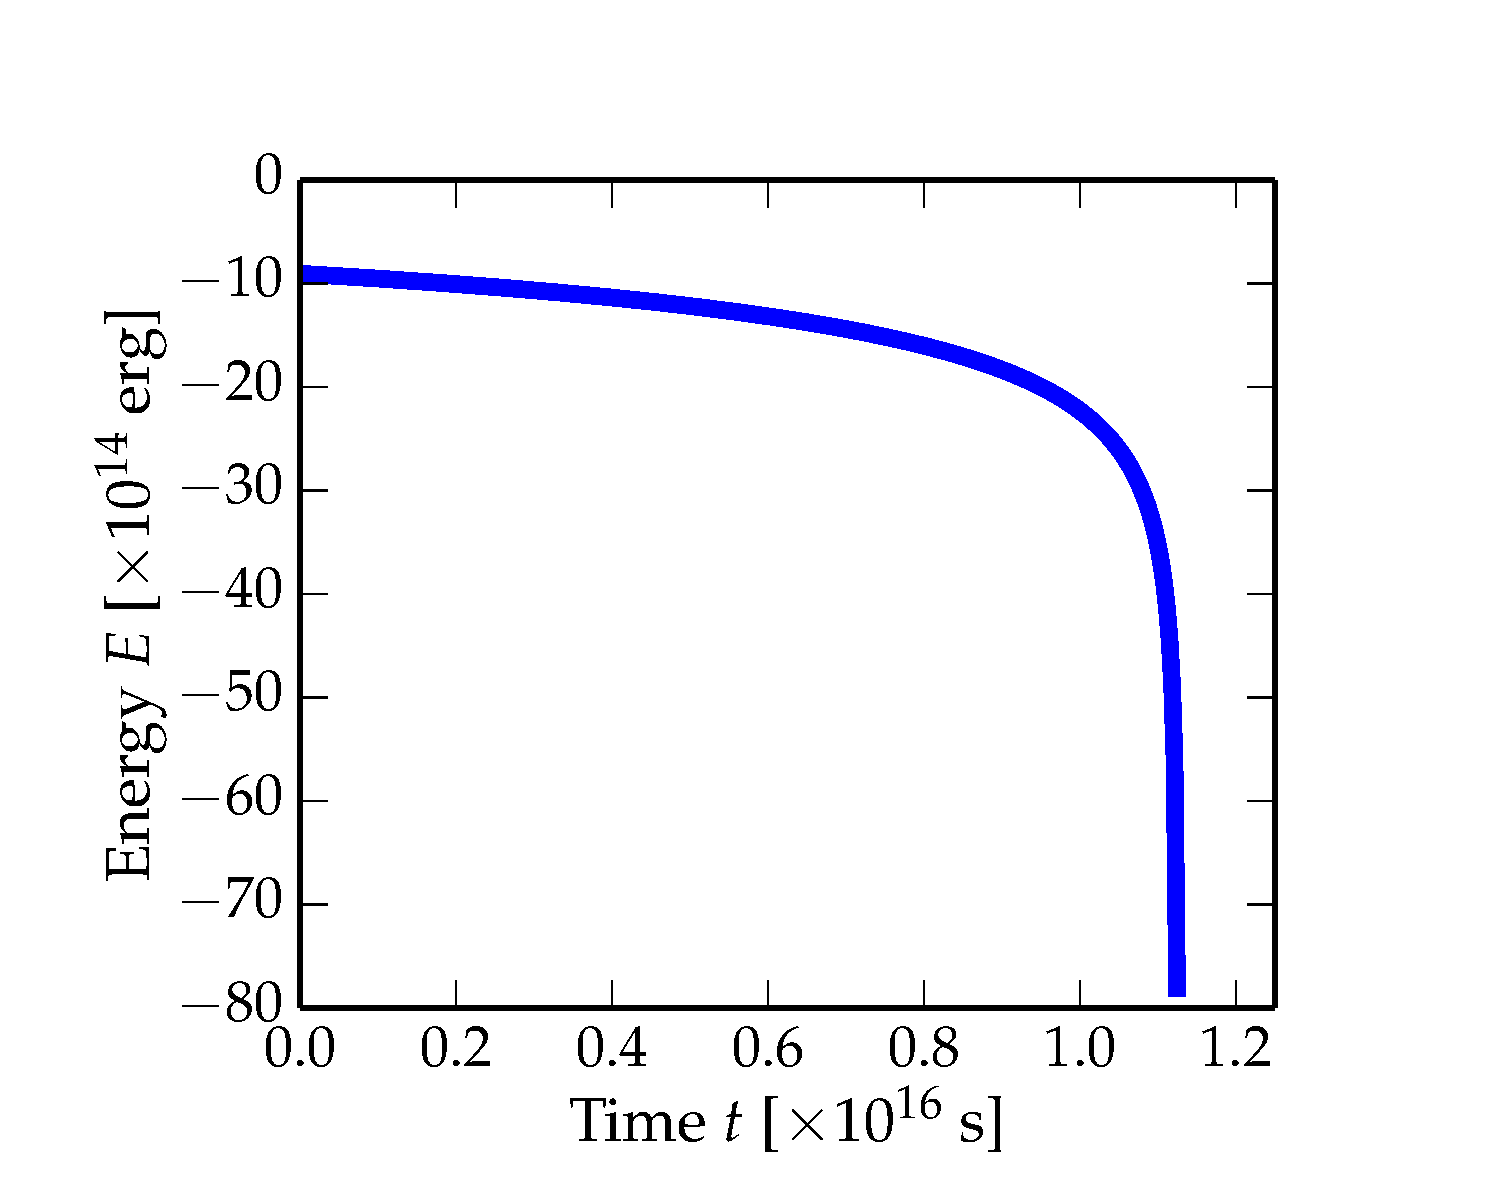
\includegraphics[width=1.2\textwidth]{billion_figs/energy.pdf}
\caption{The energy of the Hulse-Taylor binary over the course of \(\sim\) 300 million years. Energy is radiated away by gravitational waves at a rate that increases as the binary separation decreases over time.}
\label{billion-energy}
\end{figure}

\subsection{Final Inspiral of Hulse-Taylor Binary}

We proceeded to simulate the final inspiral of the Hulse-Taylor Binary in detail. The evolution of the system in its last few minutes is interesting because it is in this time that the emitted gravitational waves are in a frequency band to which interferometric gravitational wave detectors such as LIGO are sensitive. To motivate our simulation, let us analytically examine the properties of a binary to which LIGO is sensitive.

The LIGO sensitivity band is approximately 10 - 1000 Hz. The orbital frequency of a Kepler orbit of semi-major axis \(a\) is \(\nu = \frac{1}{2 \pi} \sqrt{\frac{GM}{a^3}}\), which means that a \(1.4 M_\odot - 1.4 M_\odot\) binary will produce detectable gravitational waves (noting that gravitational wave frequencies for equal-mass binaries in circular orbits are twice the orbital frequency) when its semi-major axis is in the range \(2.1 \times 10^6 - 4.6 \times 10^7\) cm. Taken together Figures~\ref{billion-axis} and~\ref{billion-ecc} assure us that by the time the semi-major axis in in that range, the eccentricity of the orbit is nearly zero, allowing us to safely make the approximation of a circular orbit.

If we make the approximation that the eccentricity~\(e = 0\) at some time \(t_0\), then Equations~\eqref{axis}~and~\eqref{ecc} can be solved exactly for \(t > t_0\). The analytical solutions are
\[ e(t) = 0 \]
\begin{equation} \label{axis-analyt}
a(t) = \left( - \frac{256}{5} \frac{G^3 m_1 m_2 M}{c^5} t \right)^{1/4}
\end{equation}
where \(t = 0\) is the time at coalescence (for times after circularization but before coalescence, \(t_0 < t < 0\)). Equation~\eqref{axis-analyt} indicates that we need to simulate starting at \(t_0 \simeq -162.6\) s in order to capture the evolution during the time it produces detectable gravitational waves.

We therefore set the initial conditions \(a_0 = 4.6 \times 10^7\) cm and \(e_0 = 0\) at \(t_0 = -162.6\) s and allowed the system to evolve until \(t = 0\).  The analytic result~\eqref{axis-analyt} for the semi-major axis is compared to the numerical result of the simulation in Figure~\ref{inspiral-axis}.

\begin{figure}[t!]
\vspace{-0.24cm}
\centering
\hspace*{-1cm}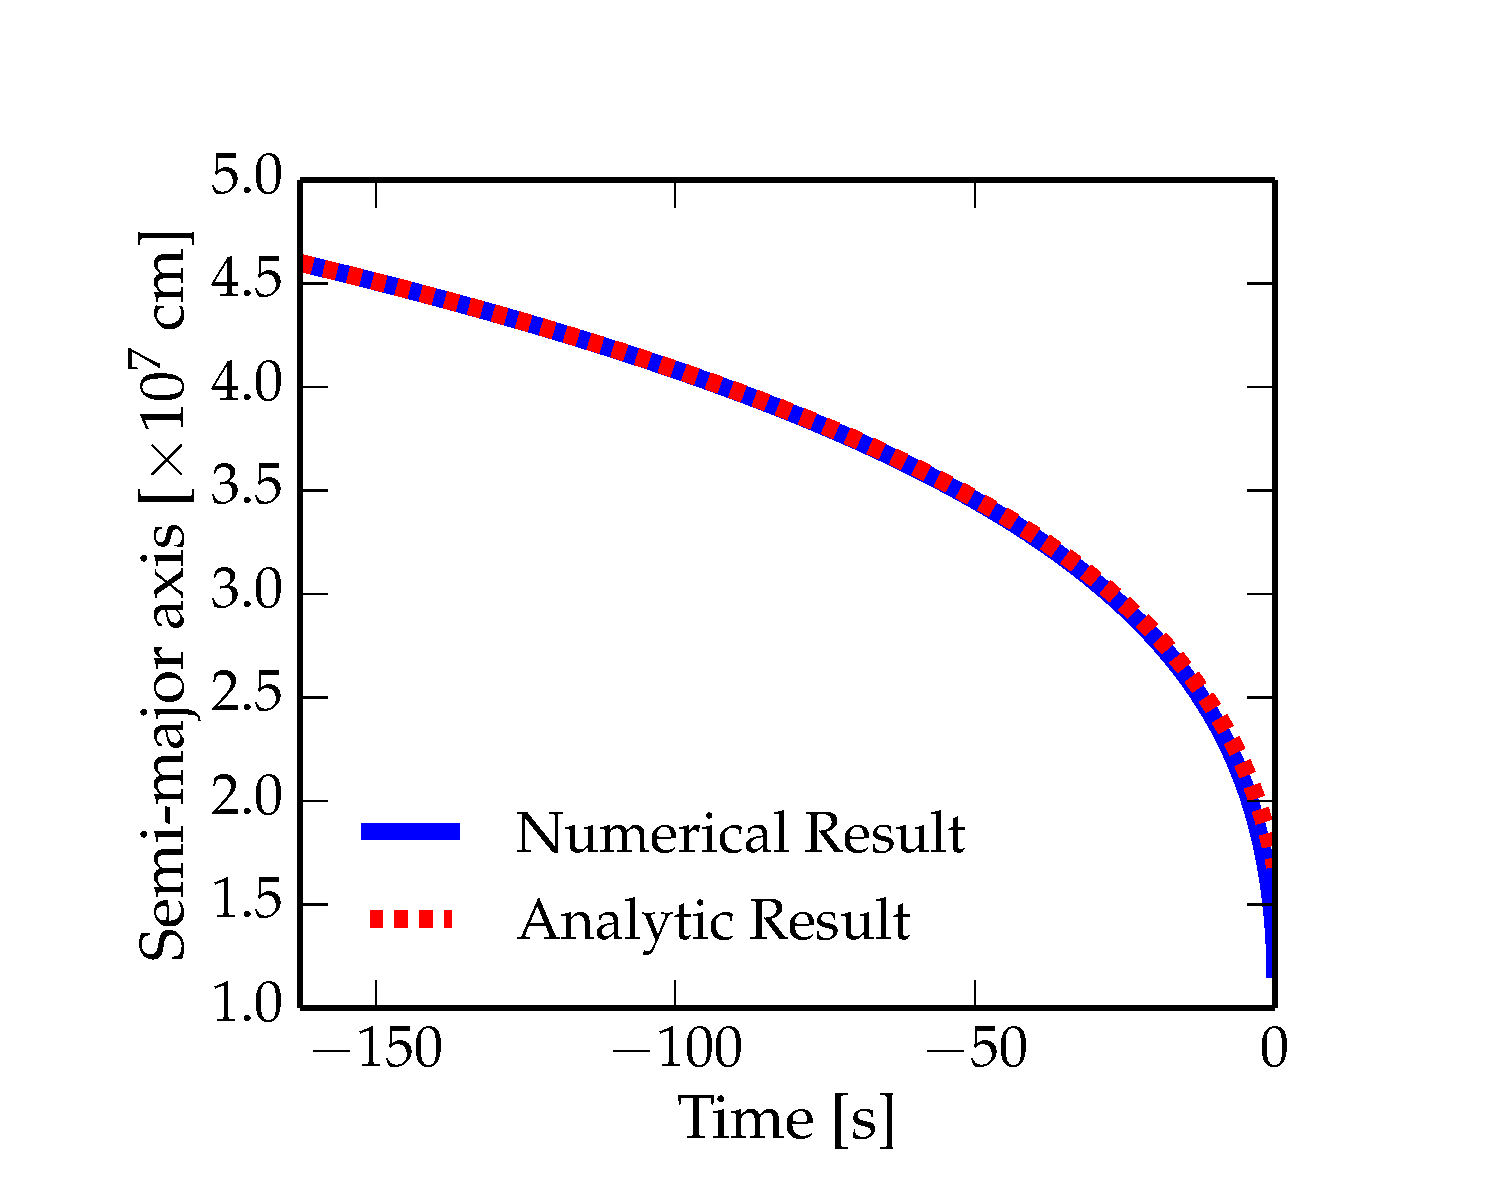
\includegraphics[width=1.2\textwidth]{inspiral_figs/inspiral_axs.pdf}
\caption{The semi-major axis of the Hulse-Taylor binary in the final few minutes before coalescence. The numerical result of the simulation is in good agreement with the analytic result~\eqref{axis-analyt}.}
\label{inspiral-axis}
\end{figure}



\begin{figure}[t!]
\vspace{-0.24cm}
\centering
\hspace*{-1cm}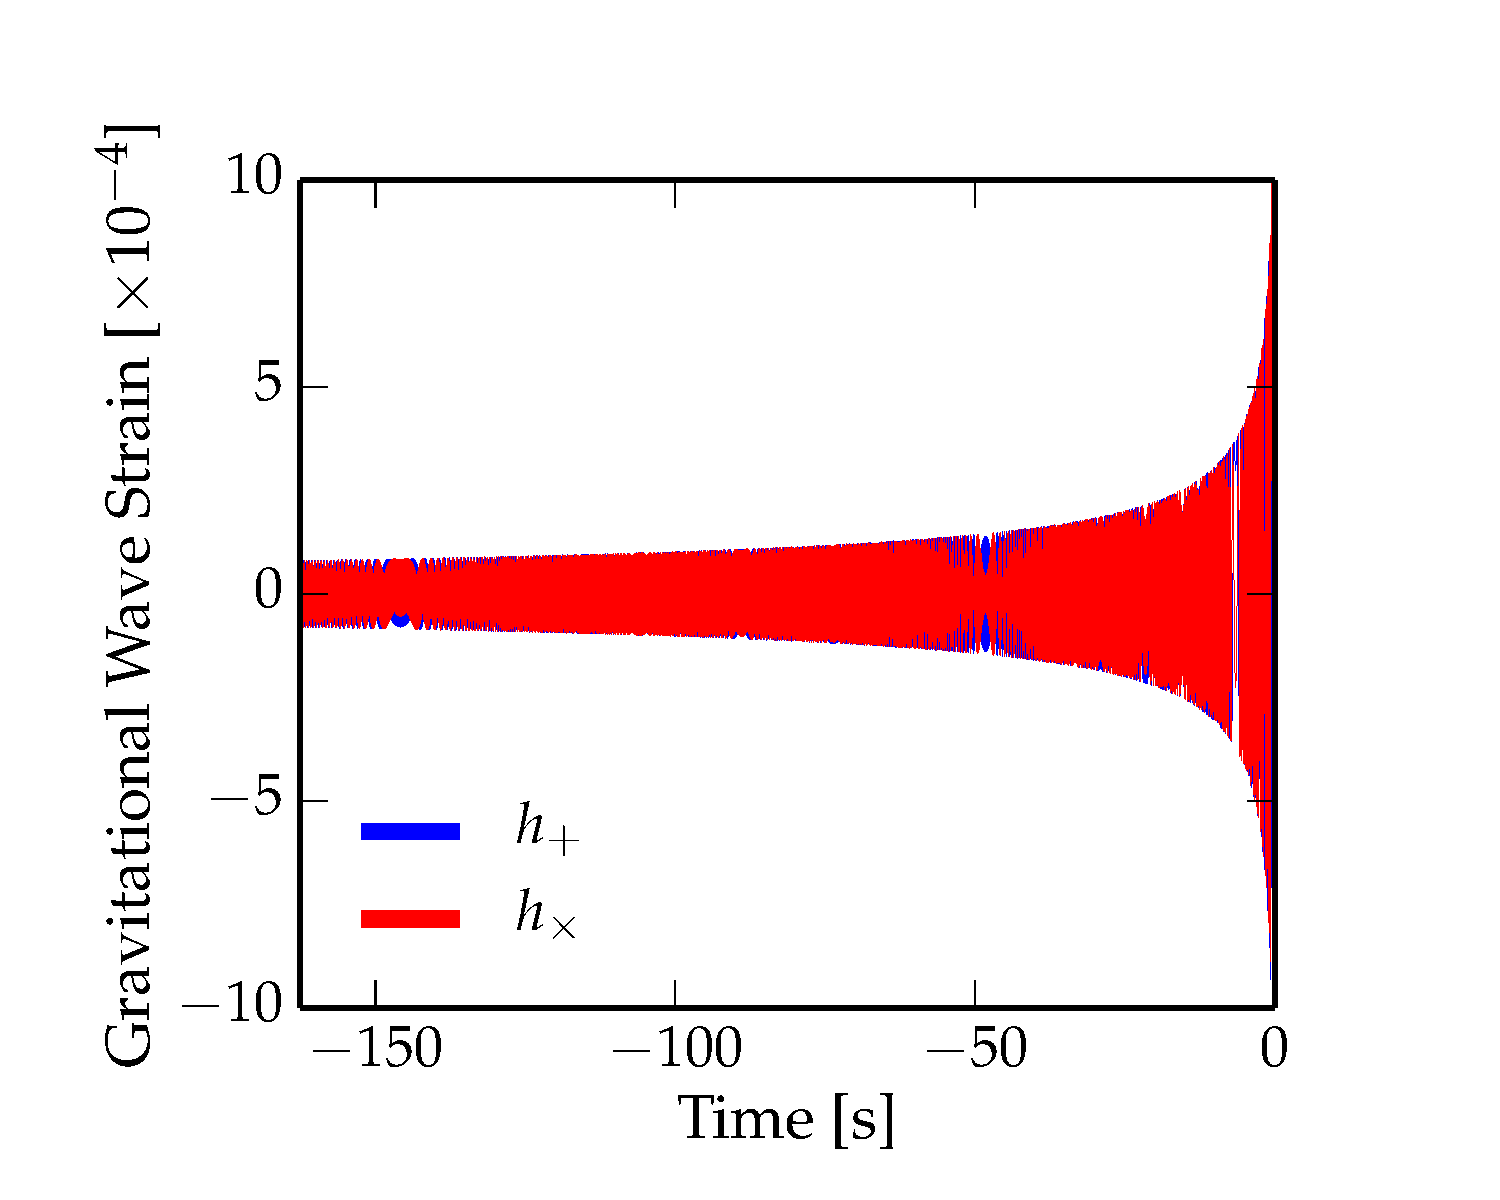
\includegraphics[width=1.2\textwidth]{inspiral_figs/inspiral_strains1.pdf}
\caption{The gravitational wave strain over the last few minutes before the Hulse-Taylor binary's coalescence. The strains oscillate too rapidly for the waveforms to be resolved in this plot, but the envelopes can be seen. Both plus and cross polarizations share the same envelope, but the cross-polarization curve largely covers the plus-polarization curve in the plot; this is an artifact of the order in which they were drawn.}
\label{inspiral-strains1}
\end{figure}

\begin{figure}[t!]
\vspace{-0.24cm}
\centering
\hspace*{-1cm}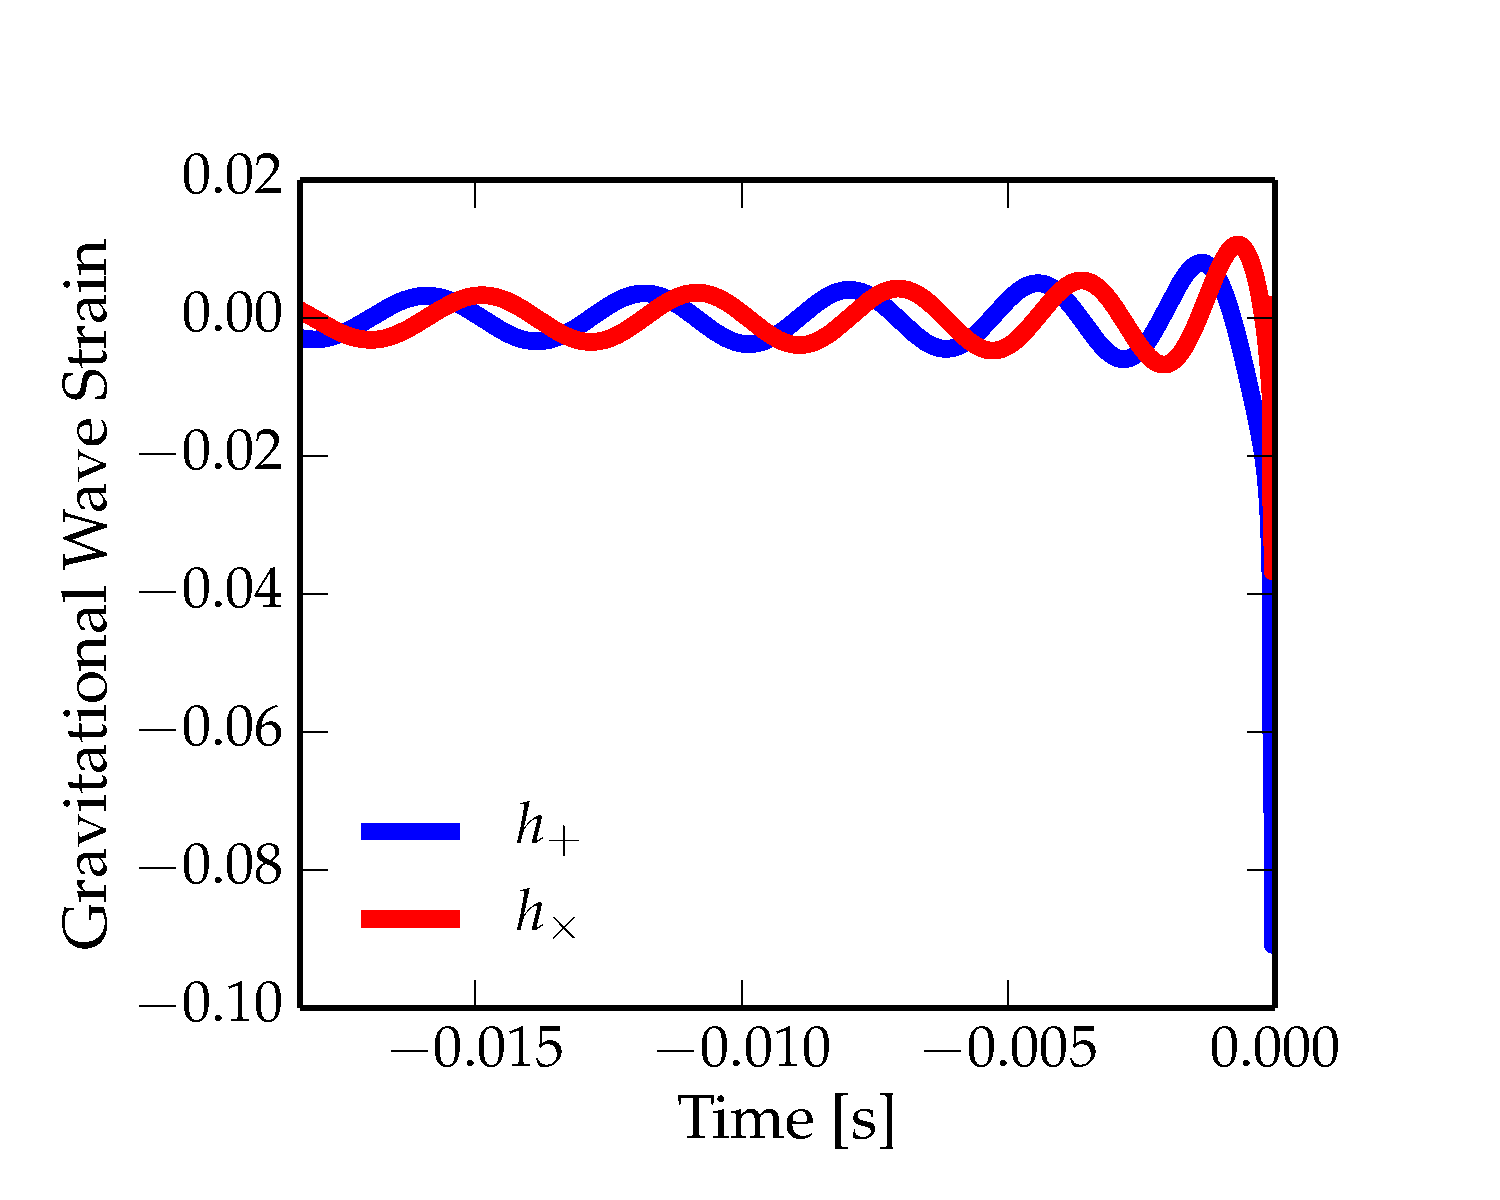
\includegraphics[width=1.2\textwidth]{inspiral_figs/inspiral_strains2.pdf}
\caption{The gravitational wave strain over the last few milliseconds before the Hulse-Taylor binary's coalescence.}
\label{inspiral-strains2}
\end{figure}

\begin{figure}[t!]
\vspace{-0.24cm}
\centering
\hspace*{-1cm}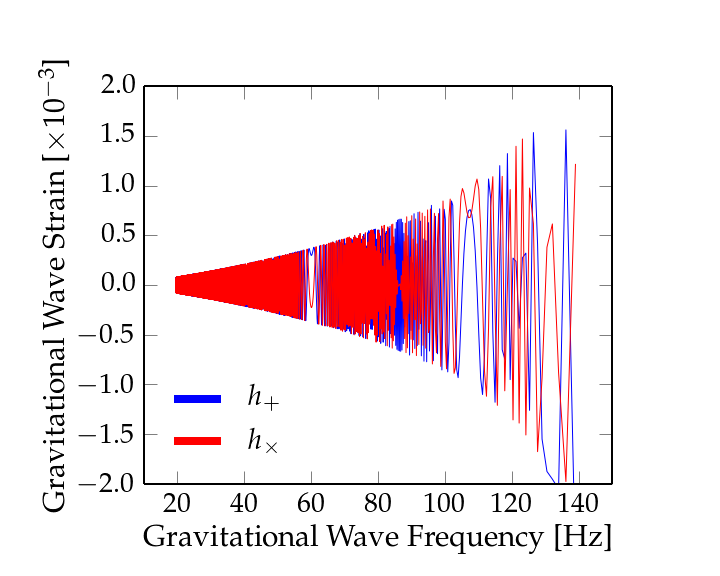
\includegraphics[width=1.2\textwidth]{inspiral_figs/inspiral_strain_spectrum.png}
\caption{The gravitational wave strain of the Hulse-Taylor binary as a function of gravitational wave frequency, which is twice the orbital frequency for equal-mass binaries with circular orbits. Comparing this plot to Figure~\ref{inspiral-strains1} reveals that gravitational wave frequencies of higher than 80 Hz only occur in the the last second of the inspiral.}
\label{inspiral-strain-spectrum}
\end{figure}

\begin{figure}[t!]
\vspace{-0.24cm}
\centering
\hspace*{-1cm}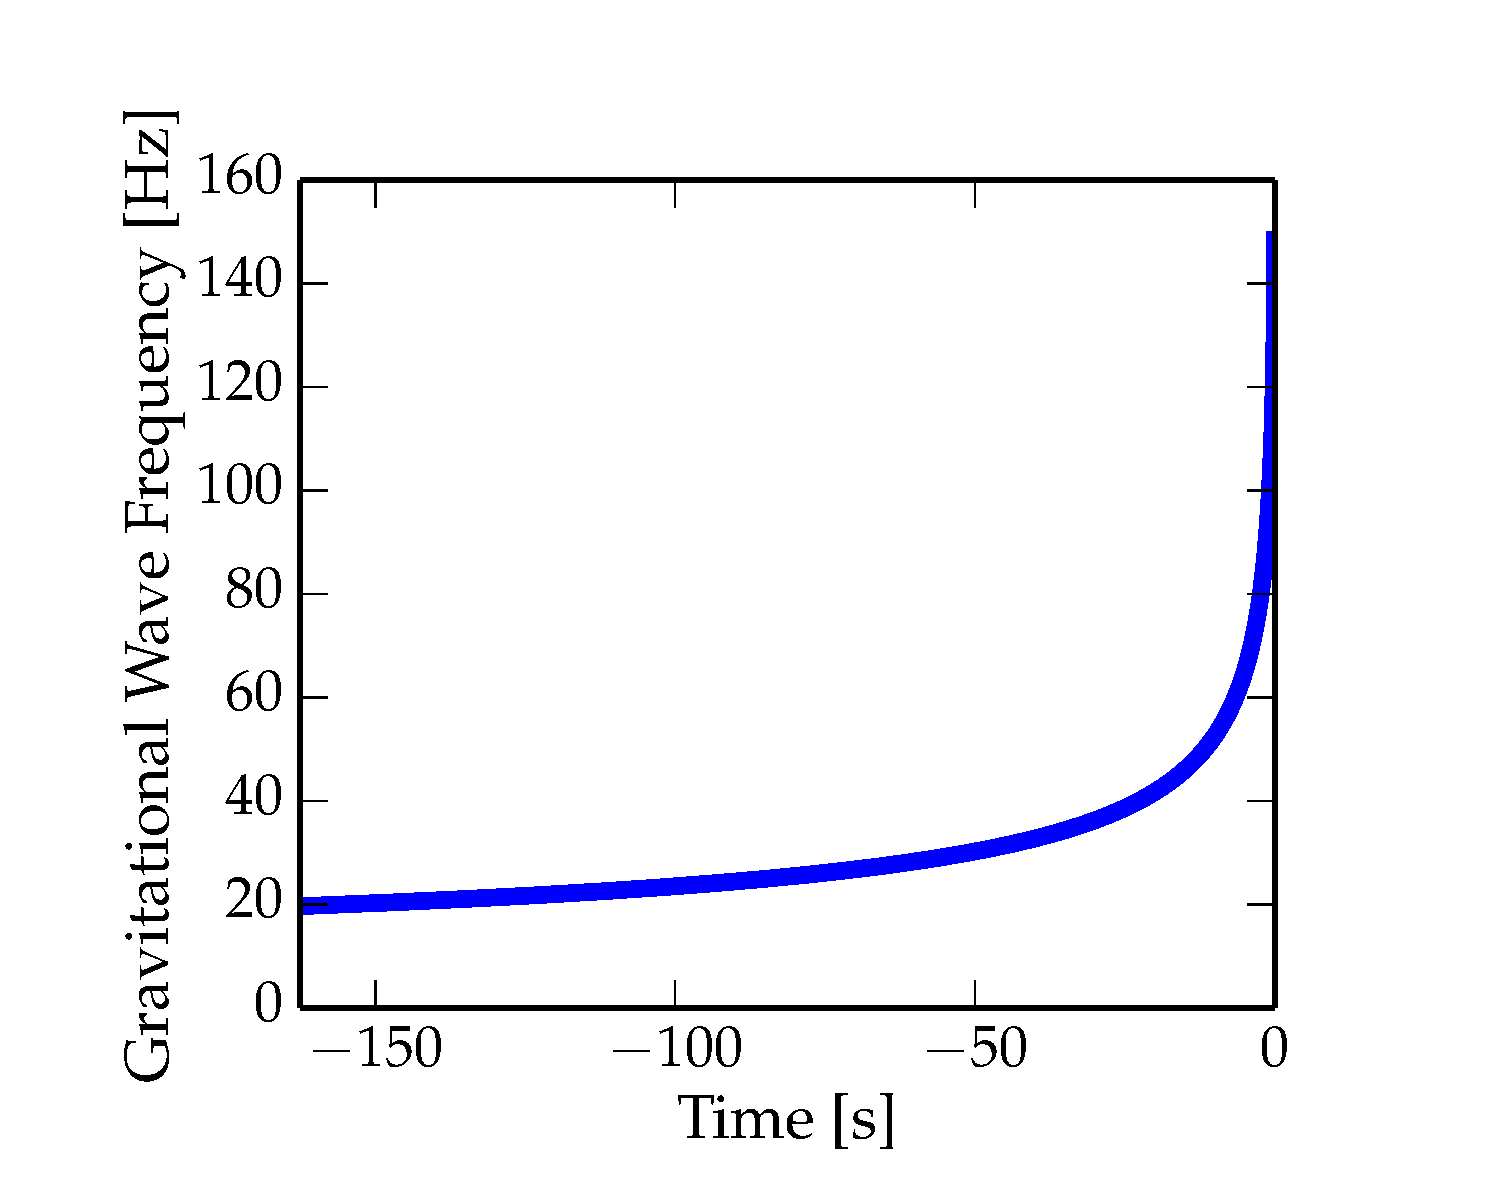
\includegraphics[width=1.2\textwidth]{inspiral_figs/inspiral_freqs.pdf}
\caption{The emitted gravitational-wave frequency over the final minutes of the Hulse-Taylor inspiral.}
\label{inspiral-gw-freq}
\end{figure}

The gravitational wave emissions of the inspiraling binary are plotted over the last few minutes in Figure~\ref{inspiral-strains1} and over the last few milliseconds in Figure~\ref{inspiral-strains2}, where the waveform over the last few orbits can be resolved. The amplitude of gravitational wave emission spikes as the neutron stars coalesce. Relevant to the search for gravitational wave signals of compact binary coalescence is the gravitational wave strain-frequency spectrum, plotted in Figure~\ref{inspiral-strain-spectrum}. Also interesting is the gravitational wave frequency as a function of time just before the coalescence, which is plotted in Figure~\ref{inspiral-gw-freq}. This is the characteristic ``sound'' of compact binary coalescences that LIGO people like to play for you.

\section{Conclusion}

Using the results of Peters 1964, one can find expressions for the rates of change of the semi-major axis and the eccentricity for a binary stellar system with respect to time. By integrating these results in a simulation using a Runge-Kutta 4 integration scheme, we are able to accurately recreate the predicted inspiral of such a binary system.

Having developed an accurate means for determining the orbits of a binary system, the simulation can then be applied to studying the gravitational wave emission of an coalescing binary. The final regime of the inspiral can be compared to what is found analytically when the eccentricity is approximated to be zero, and the gravitational wave emission can be characterized for use in gravitational wave detection.

%%%%%%%%%%%
\end{document}
